\documentclass{beamer}
\usepackage{graphics}
\usepackage{epsfig}
\usepackage{multicol}
\setbeamertemplate{navigation symbols}{}
\newcommand{\RR}{\ensuremath{\mathbb{R}}}
\newcommand{\NN}{\ensuremath{\mathbb{N}}}
\newcommand{\QQ}{\ensuremath{\mathbb{Q}}}
\newcommand{\CC}{\ensuremath{\mathbb{C}}}
\newcommand{\ZZ}{\ensuremath{\mathbb{Z}}}
\newcommand{\TT}{\ensuremath{\mathbb{T}}}
\newcommand{\HH}{\ensuremath{\mathbb{H}}}
\DeclareMathOperator{\Min}{Min}
\DeclareMathOperator{\Dom}{Dom}
\DeclareMathOperator{\vol}{vol}
\DeclareMathOperator{\Aut}{Aut}
\DeclareMathOperator{\Stab}{Stab}
\DeclareMathOperator{\Sym}{Sym}
\DeclareMathOperator{\Grp}{Grp}
\DeclareMathOperator{\HYP}{HYP}
\DeclareMathOperator{\CUT}{CUT}
\DeclareMathOperator{\GL}{GL}
\DeclareMathOperator{\AGL}{AGL}
\DeclareMathOperator{\Id}{Id}
\DeclareMathOperator{\vertt}{vert}
\DeclareMathOperator{\conv}{conv}
\DeclareMathOperator{\rank}{rank}

\def\QuotS#1#2{\leavevmode\kern-.0em\raise.2ex\hbox{$#1$}\kern-.1em/\kern-.1em\lower.25ex\hbox{$#2$}}

\begin{document}
\title{The parametrization of fullerenes}
\author{
{\small
\begin{center}
\textcolor{red}{\large Mathieu Dutour Sikiri\'c}\\[2mm]
\textcolor{red}{Rudjer Bo\u skovi\'c Institute, Croatia}
\end{center}
}
}
\date{\today} 
\frame{\titlepage} 





\frame{
\begin{center}
{\Huge 
\begin{tabular*}{6cm}{c}
\\[-0.5cm]
\textcolor{blue}{I. }\textcolor{red}{Fullerenes}\\
\end{tabular*}
}
\end{center}
}


\frame{
  \frametitle{Fullerenes}


\begin{itemize}
\item A fullerene is a $3$-valent plane graph, whose faces are $5$ or $6$-gonal.
\item They exist for any even $n\geq 20$, $n\not= 22$.
\begin{center}
%\begin{minipage}[b]{2.3cm}
%\centering
%\resizebox{20mm}{!}{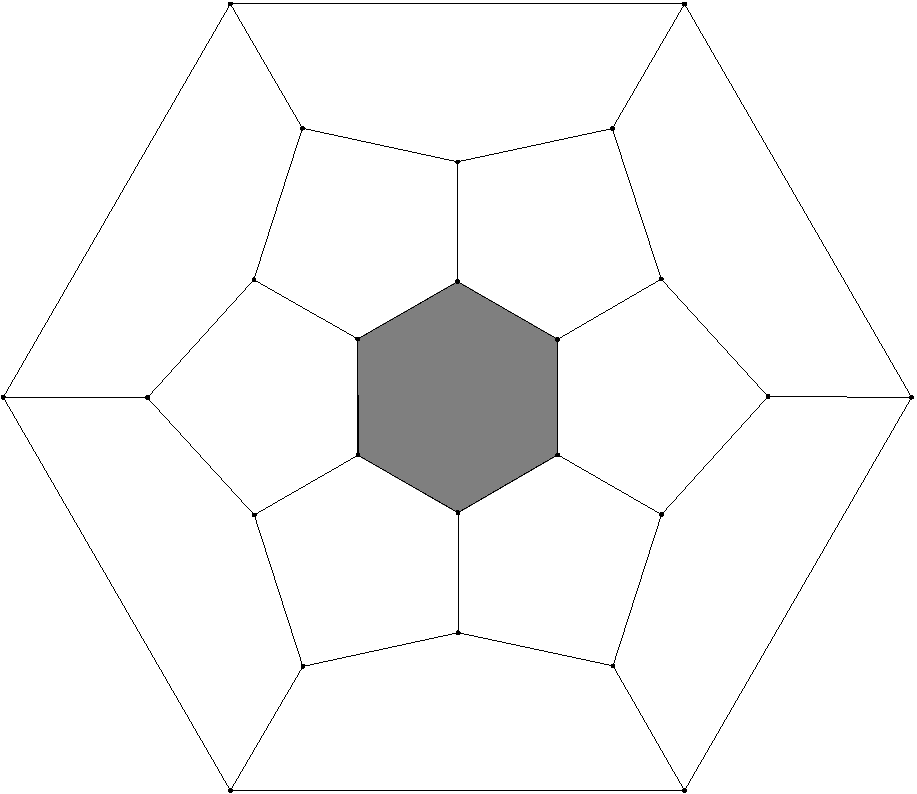
\includegraphics[bb=1 1 440 381, clip]{PictureAppli/F2sec.pdf}}\par
%24
%\end{minipage}
%\begin{minipage}[b]{2.3cm}
%\centering
%\resizebox{20mm}{!}{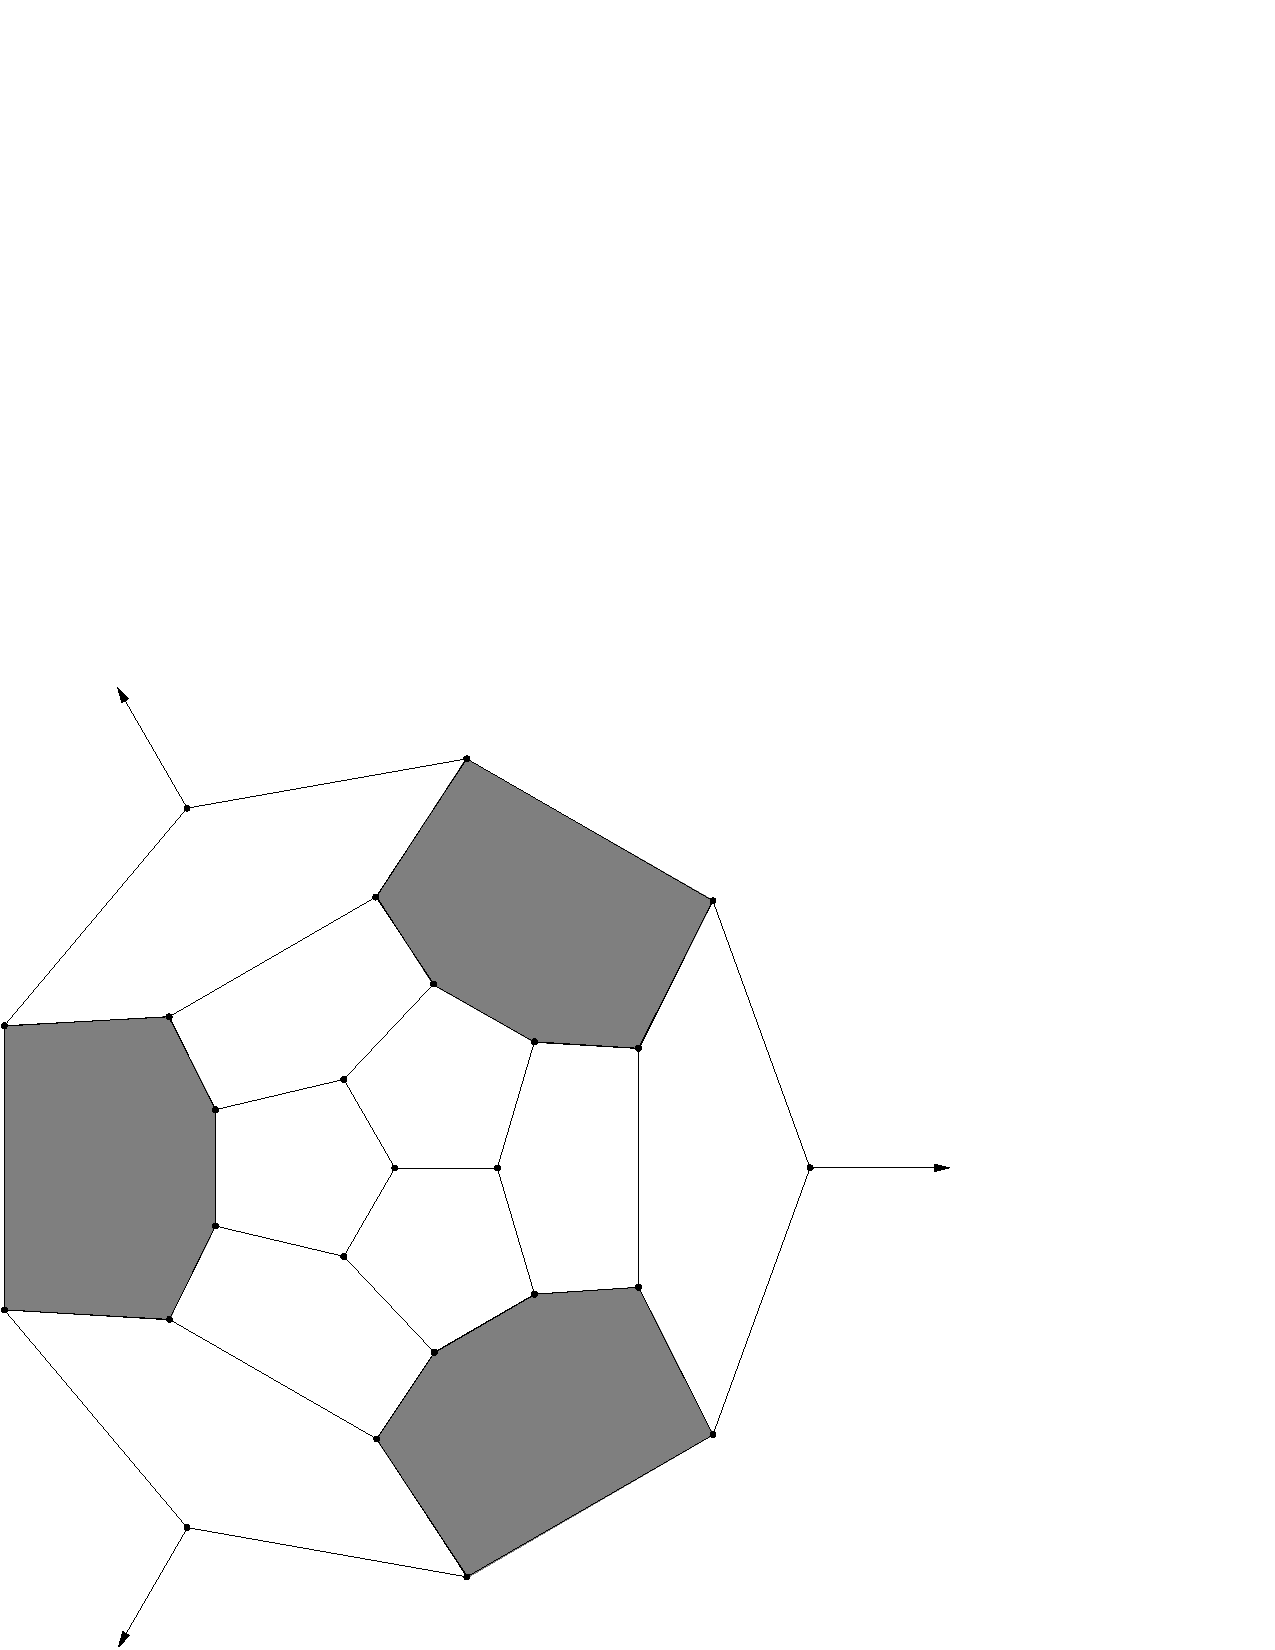
\includegraphics[bb=1 1 457 464, clip]{FullPresPic/Picture2.pdf}}\par
%26
%\end{minipage}
\begin{minipage}[b]{2.3cm}
\centering
\resizebox{13mm}{!}{\rotatebox{90}{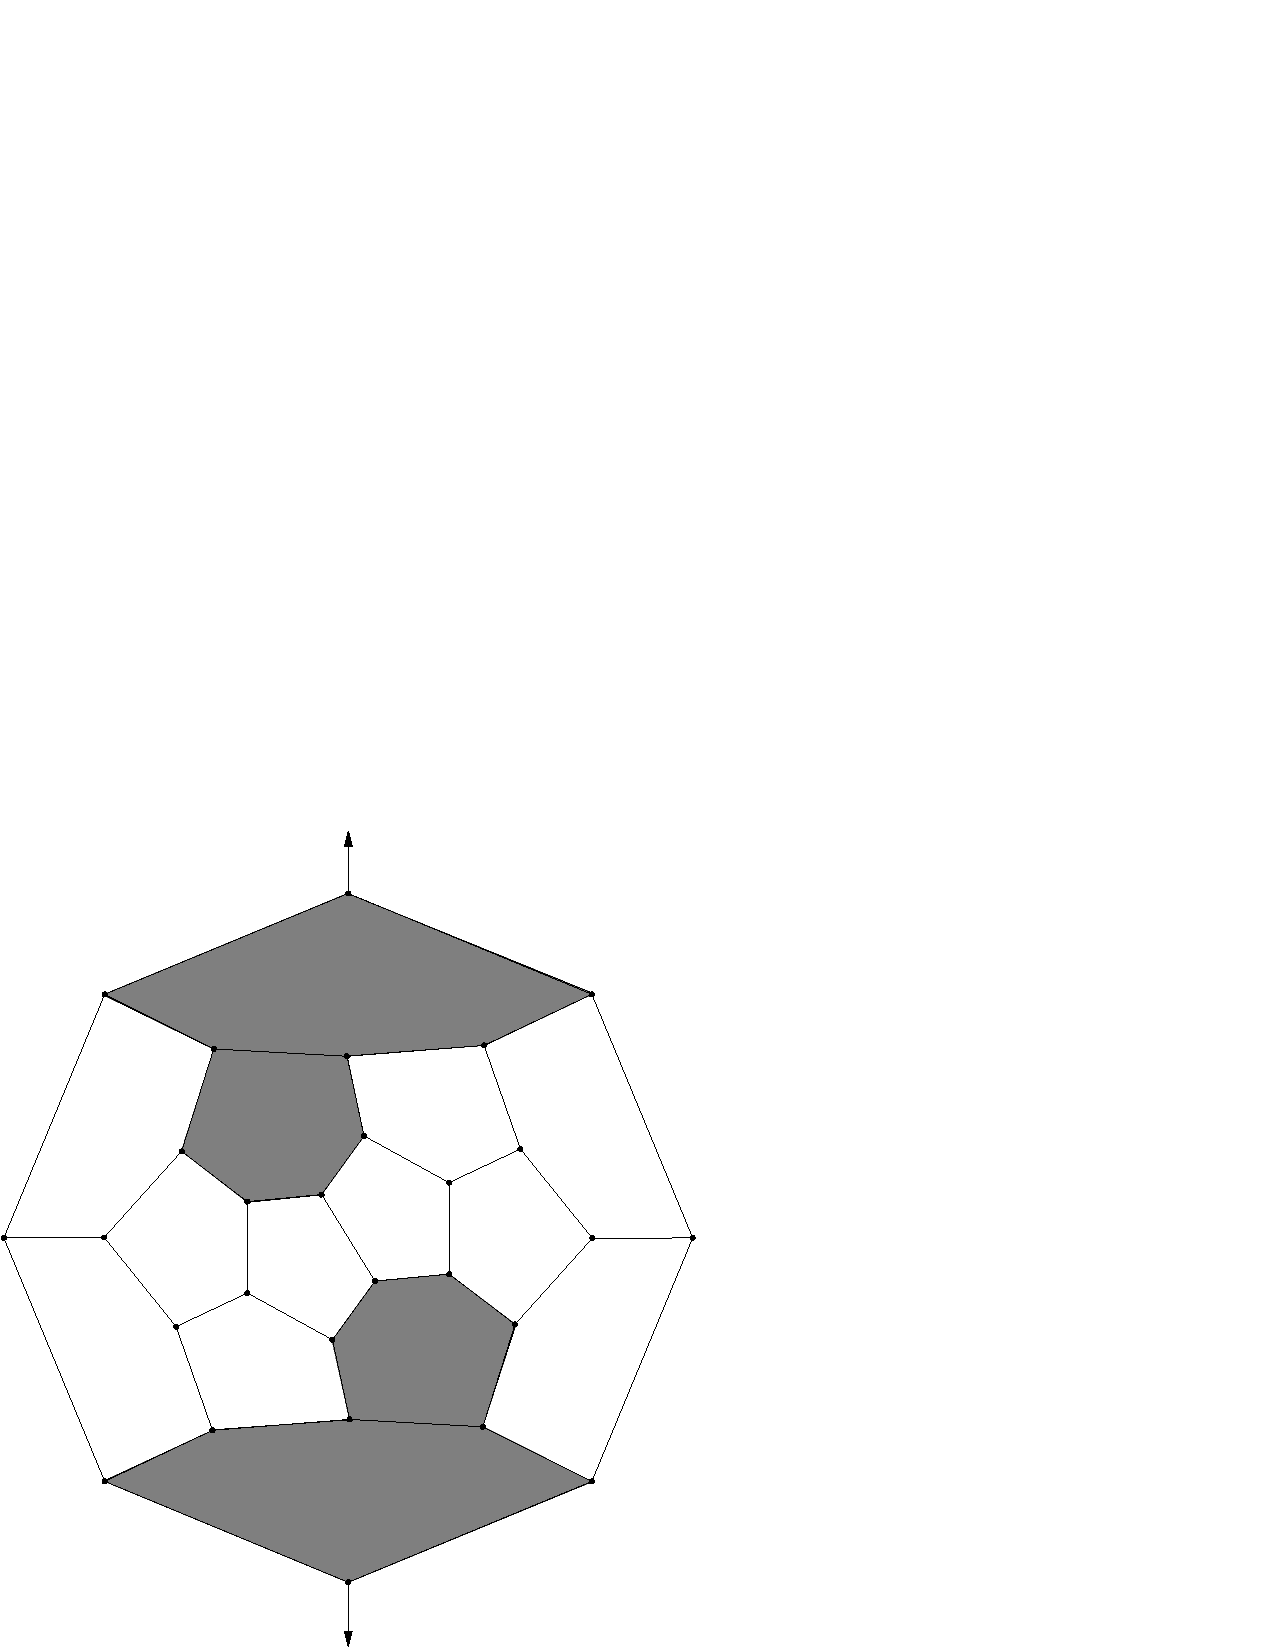
\includegraphics[bb=1 1 333 395, clip]{FullPresPic/Picture3.pdf}}}\par
\end{minipage}
%\begin{minipage}[b]{2.3cm}
%\centering
%\resizebox{20mm}{!}{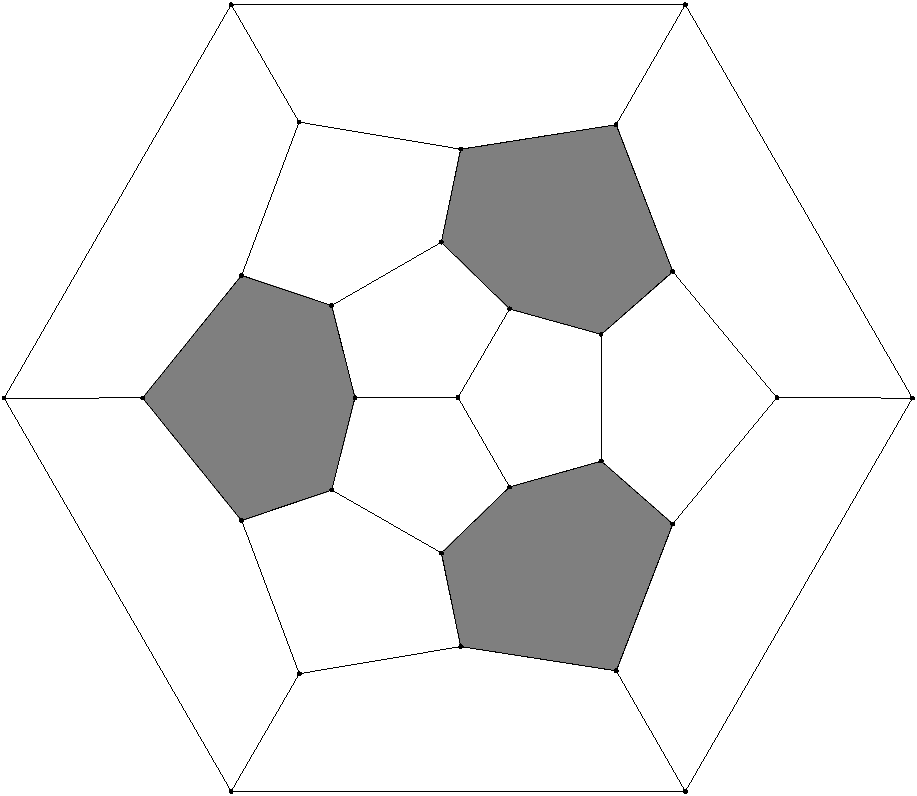
\includegraphics[bb=1 1 439 380, clip]{PictureAppli/F4sec.pdf}}\par
%28
%\end{minipage}
\begin{minipage}[b]{2.3cm}
\centering
\resizebox{11mm}{!}{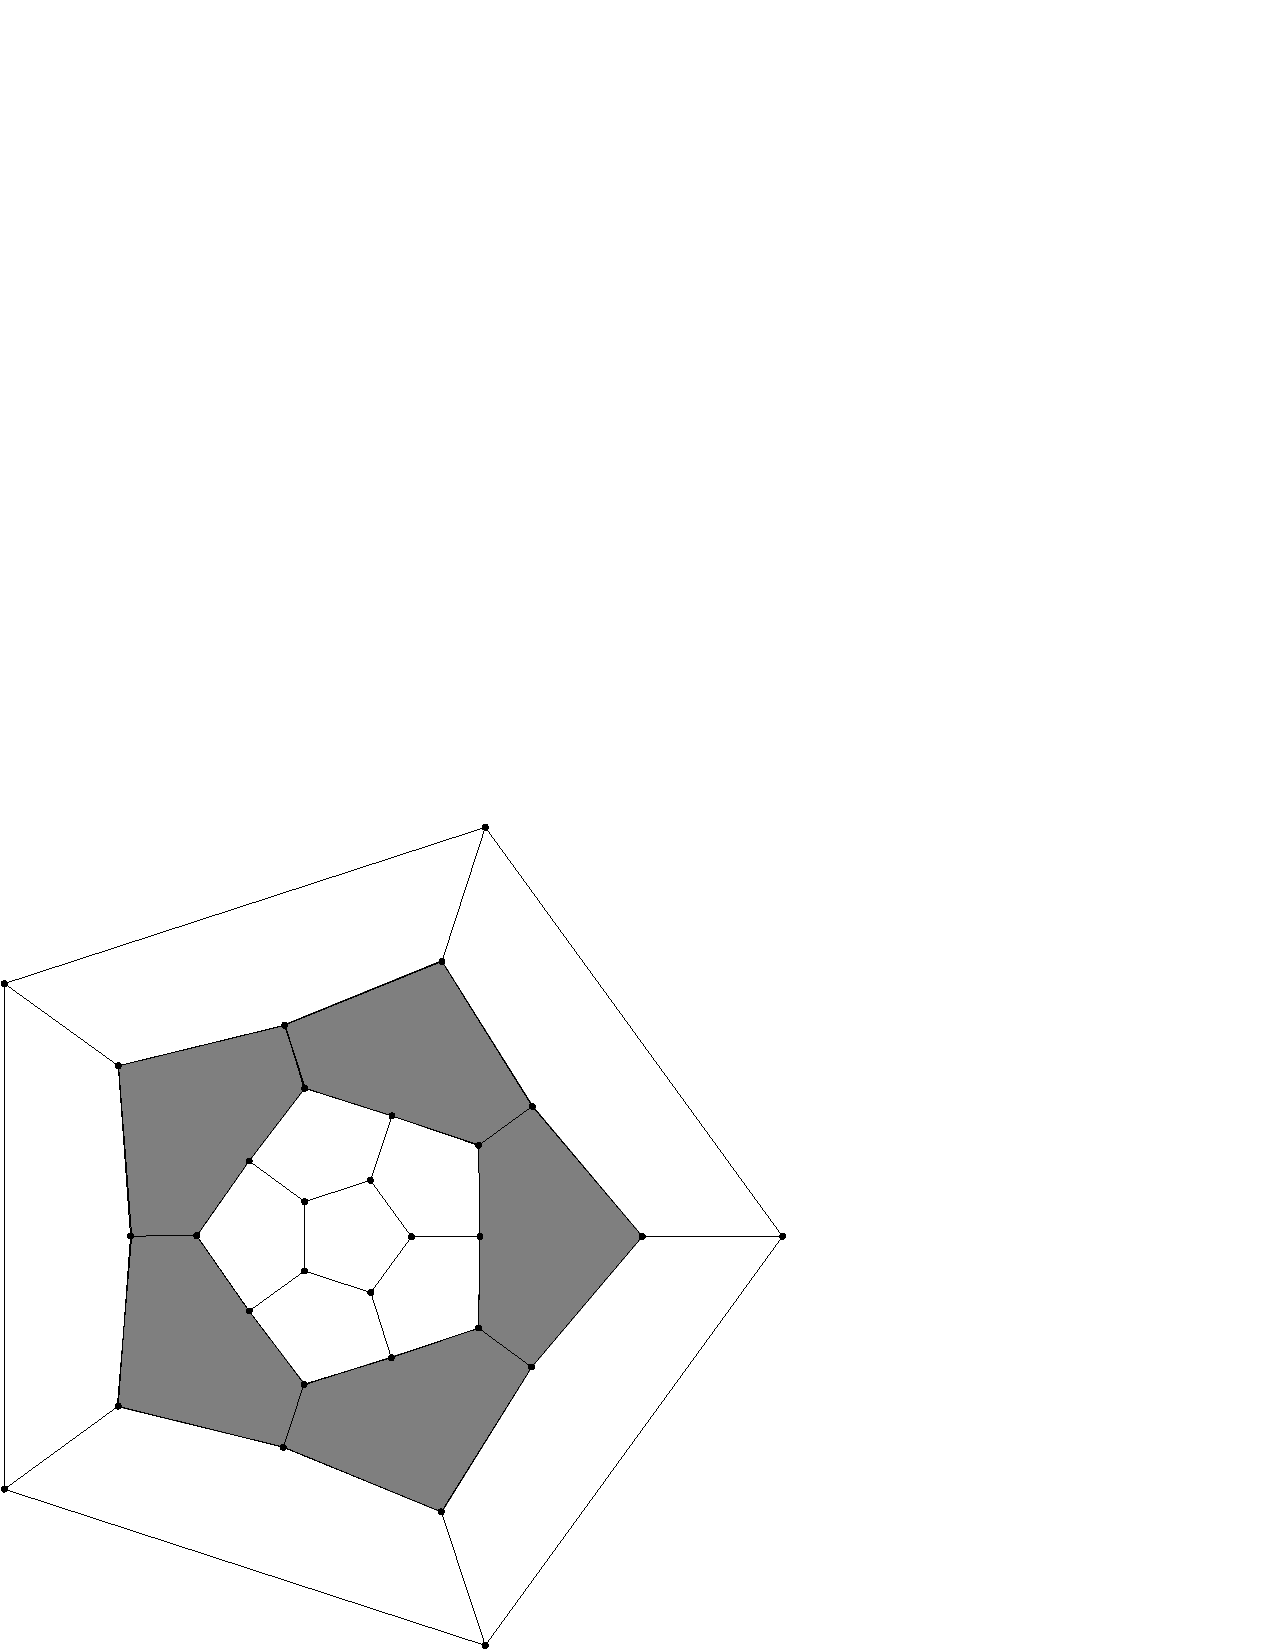
\includegraphics[bb=1 1 377 398, clip]{FullPresPic/Picture5.pdf}}\par
\end{minipage}
\begin{minipage}[b]{2.3cm}
\centering
\resizebox{13mm}{!}{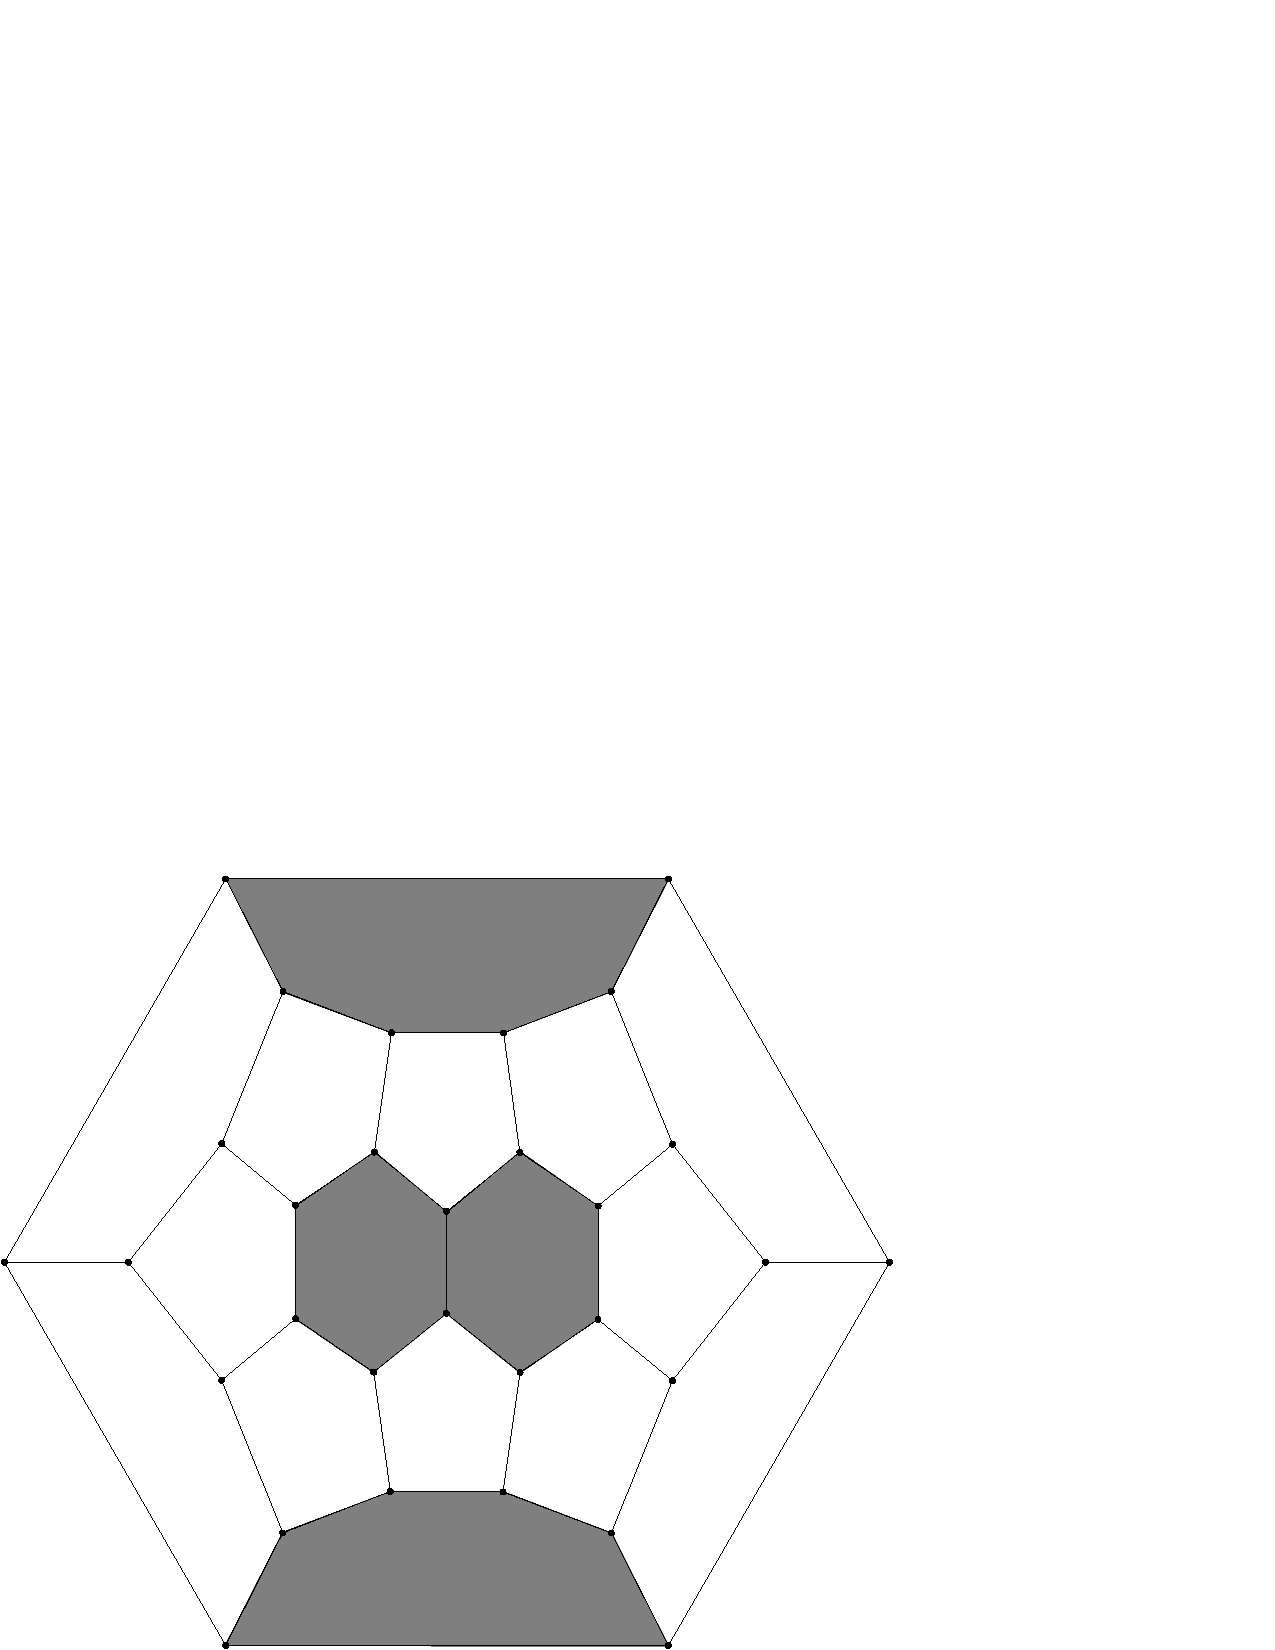
\includegraphics[bb=1 1 429 374, clip]{FullPresPic/Picture6.pdf}}\par
\end{minipage}
\begin{minipage}[b]{2.3cm}
\centering
\resizebox{13mm}{!}{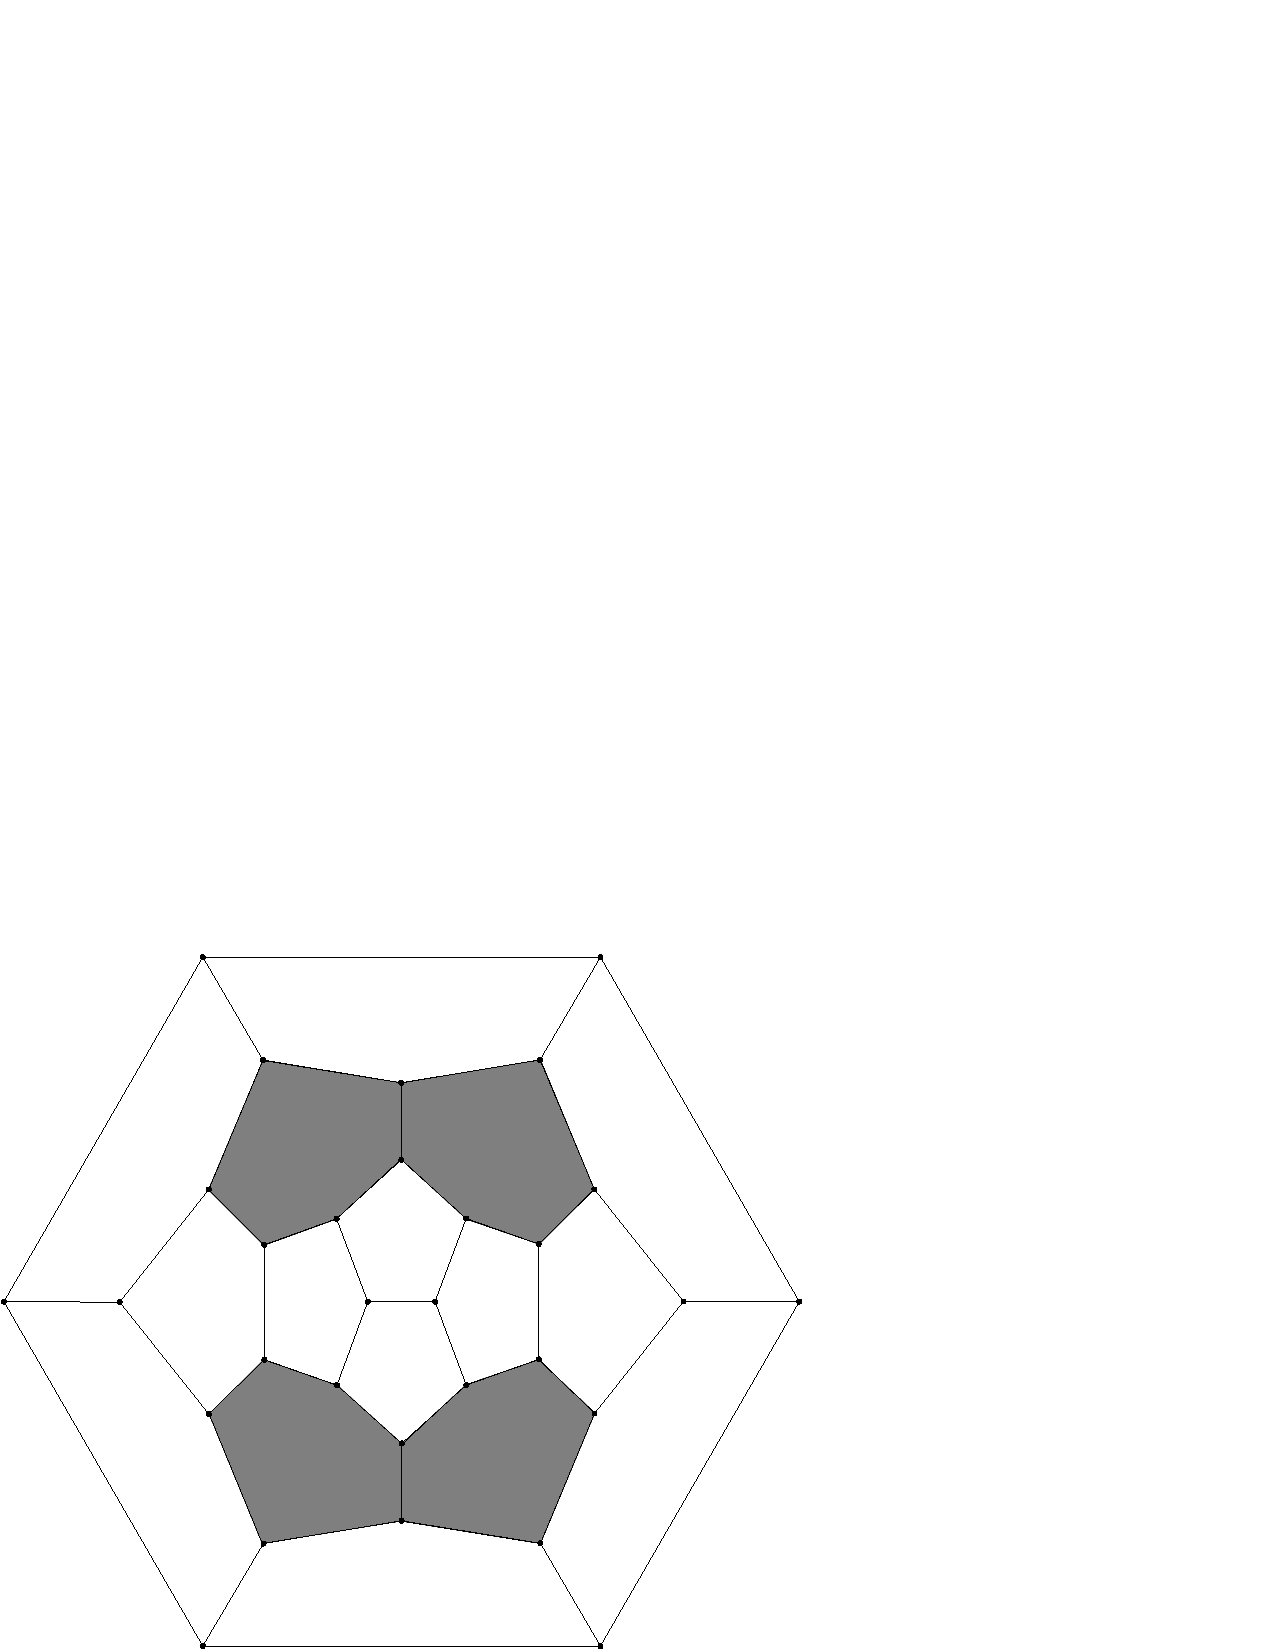
\includegraphics[bb=1 1 385 335, clip]{FullPresPic/Picture7.pdf}}\par
\end{minipage}
\end{center}
\item There exist extremely efficient programs to enumerate them (\textcolor{red}{FullGen} by G. Brinkman, \textcolor{red}{CPF} by T. Harmuth)
\item Fullerenes with isolated pentagons have $n\geq 60$. The smallest one:
\begin{center}
\begin{minipage}{4.5cm}
\centering
\resizebox{30mm}{!}{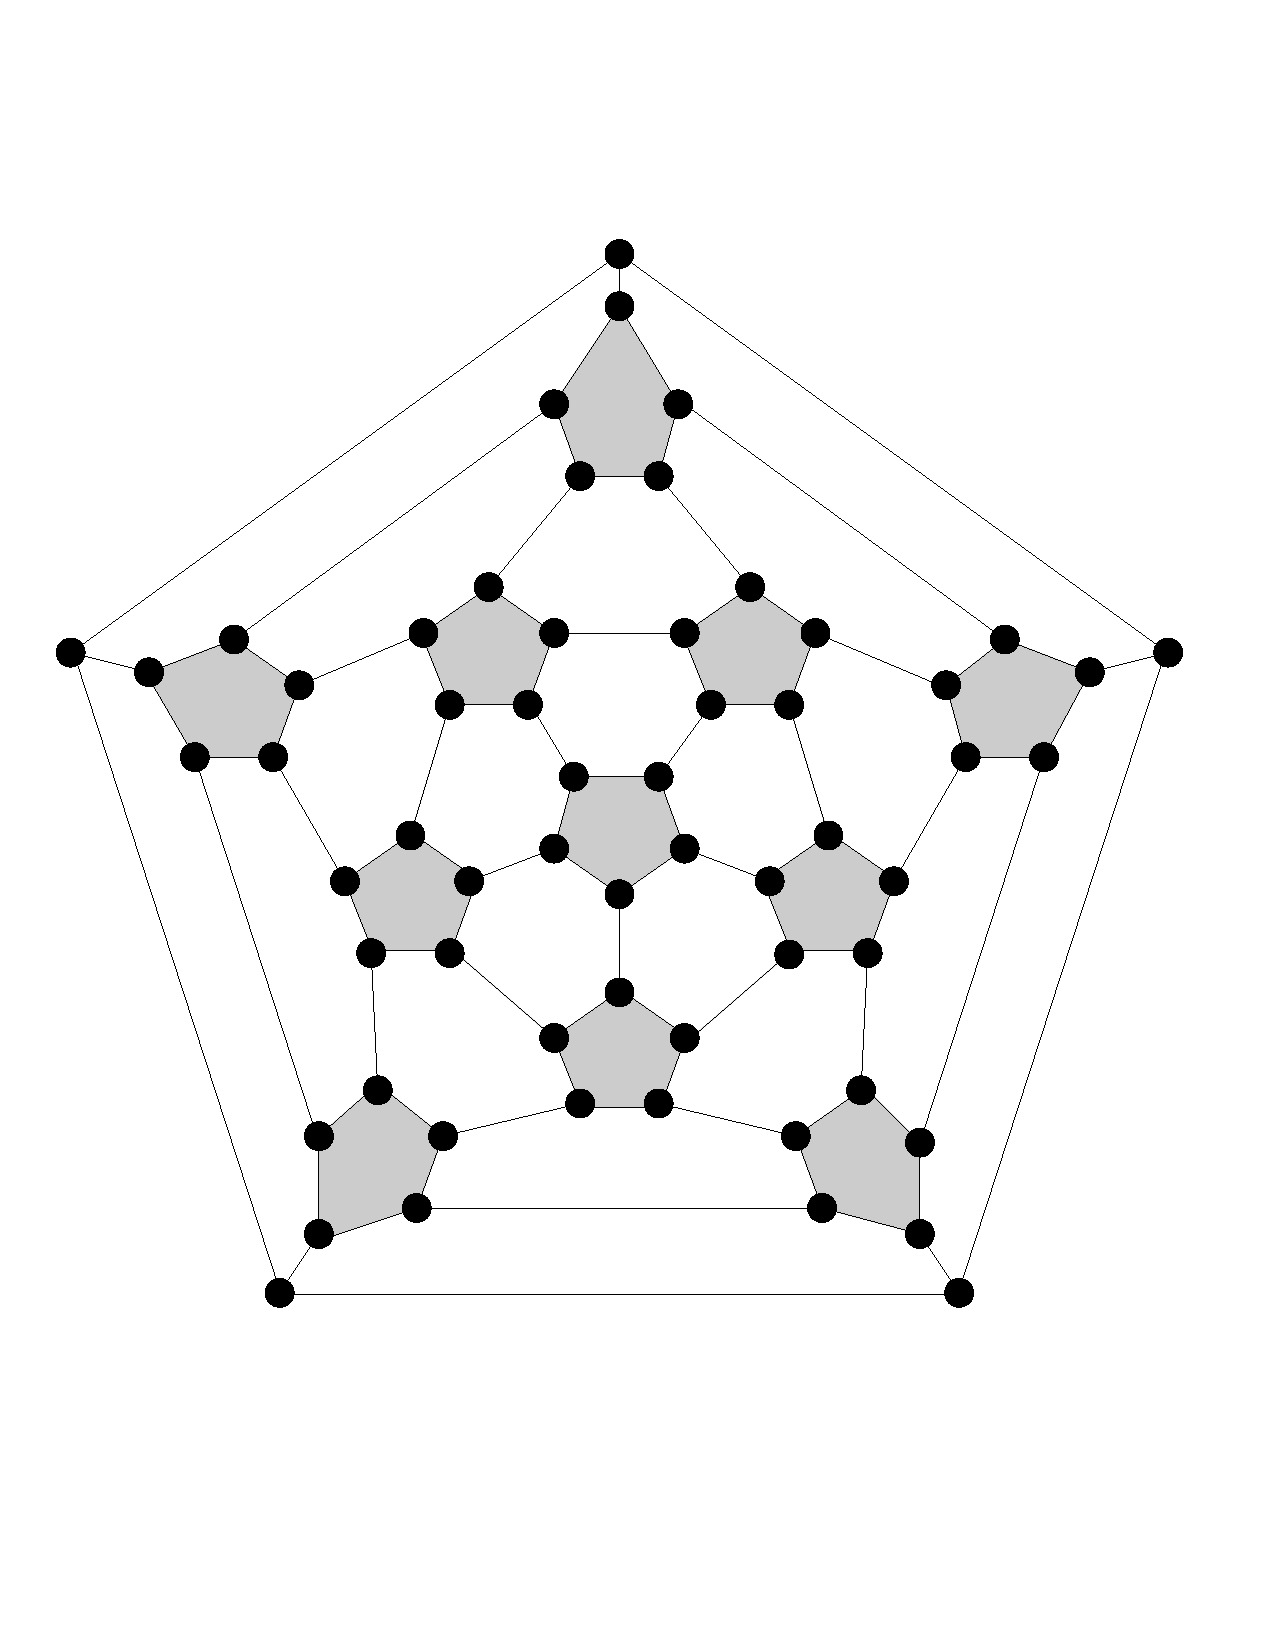
\includegraphics[bb=26 165 568 678, clip]{DRAW/PS/C60.pdf}}\par
\end{minipage}
\begin{minipage}{4.5cm}
\centering
{\em Truncated icosahedron},\par
{\em soccer ball},\par
{\em Buckminsterfullerene}
\end{minipage}



\end{center}
\end{itemize}
}


\frame{
  \frametitle{Euler formula and positive curvature}

\begin{itemize}
\item For a $3$-valent plane graph Euler formula can be rewritten as
\begin{equation*}
\sum_{i\geq 3} (6-i) p_i = 12
\end{equation*}
with $p_i$ the number of $i$-gons.
\item We restrict ourselves to graphs of \textcolor{red}{positive curvature}, i.e. those with $c_i=6-i\geq 0$. 
\item Thus we have the following possibilities for $(p_3, p_4, p_5)$:
\begin{equation*}
\begin{array}{ccccc}
\textcolor{red}{(0,0,12)} & (0,1,10) & (0,2,8) & (0,3,6) & (0,4,4)\\
(0,5,2)  & \textcolor{red}{(0,6,0)} & (1,0,9) & (1,1,7)  & (1,2,5)\\
(1,3,3) & (1,4,1) & (2,0,6)  & (2,1,4)  & (2,2,2)\\
(2,3,0) & (3,0,3)  & (3,1,1)  & \textcolor{red}{(4,0,0)}&
\end{array}
\end{equation*}
\item The goal is to try to understand how one can describe such graphs:
\begin{itemize}
\item W.P. Thurston, {\em Shapes of polyhedra and triangulations of the sphere},
The Epstein birthday schrift,  511--549 (electronic),
Geom. Topol. Monogr., 1, Geom. Topol. Publ., Coventry, 1998.
\end{itemize}

\end{itemize}
}






\frame{
  \frametitle{Symmetry groups and number of fullerenes}

\begin{itemize}
\item The possible symmetry groups of fullerenes are
\begin{center}
\begin{tabular}{|c|c|c|}
\hline
class & all group                & \# param\\
\hline
$C_1$        & $C_1$, $C_s$, $C_i$       & $10$\\
$C_2$        & $C_2$, $C_{2h}$, $C_{2v}$ & $6$\\
$C_3$        & $C_3$, $C_{3h}$, $C_{3v}$ & $4$\\
$D_2$        & $D_2$, $D_{2h}$, $D_{2d}$ & $4$\\
$D_3$        & $D_3$, $D_{3h}$, $D_{3d}$ & $3$\\
$D_5$        & $D_5$, $D_{5h}$, $D_{5d}$ & $2$\\
$D_6$        & $D_6$, $D_{6h}$, $D_{6d}$ & $2$\\
$T$          & $T$, $T_{h}$, $T_{d}$     & $2$\\
$I$          & $I$, $I_{h}$              & $1$\\
\hline
\end{tabular}
\end{center}
\item The number of fullerene grows polynomially with the number of vertices.
\item The goal is to describe the fullerenes by those parameters.
\end{itemize}
}


\frame{
\begin{center}
{\Huge 
\begin{tabular*}{9cm}{c}
\\[-0.5cm]
\textcolor{blue}{II. }\textcolor{red}{Simple parameterizations}\\
\end{tabular*}
}
\end{center}
}



\frame{
  \frametitle{The case of $1$ parameter: Goldberg-Coxeter construction}

\begin{itemize}
\item Take a $3$-valent plane graph $G_0$ and two parameters $k,l\geq 0$.
\item The graph $G_0^{*}$ is a triangulation.
\item Break the triangles of $G_0^*$ into smaller triangles:
\end{itemize}
\begin{center}
\resizebox{33mm}{!}{\rotatebox{0}{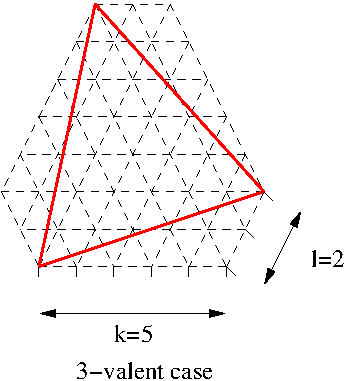
\includegraphics{GOLDBERGpicture/GoldbergBreakdown3val.pdf}}}\par
\end{center}
\begin{itemize}
\item Glue all those pices together and get another triangulation
\item Take the dual and get a $3$-valent plane graph $GC_{k,l}(G_0)$.
\end{itemize}

}

\frame{
  \frametitle{Example of $GC_{2,1}(Cube)$}
\begin{center}
\resizebox{90mm}{!}{\rotatebox{0}{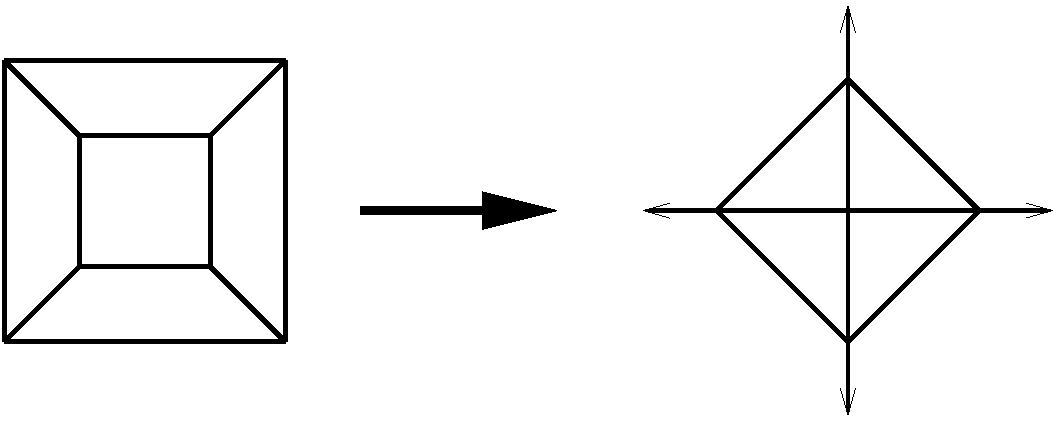
\includegraphics{GOLDBERGpicture/CubeSec.pdf}}}\par
\end{center}
}

\frame{
  \frametitle{Example of $GC_{2,1}(Cube)$}
\begin{center}
\resizebox{97mm}{!}{\rotatebox{0}{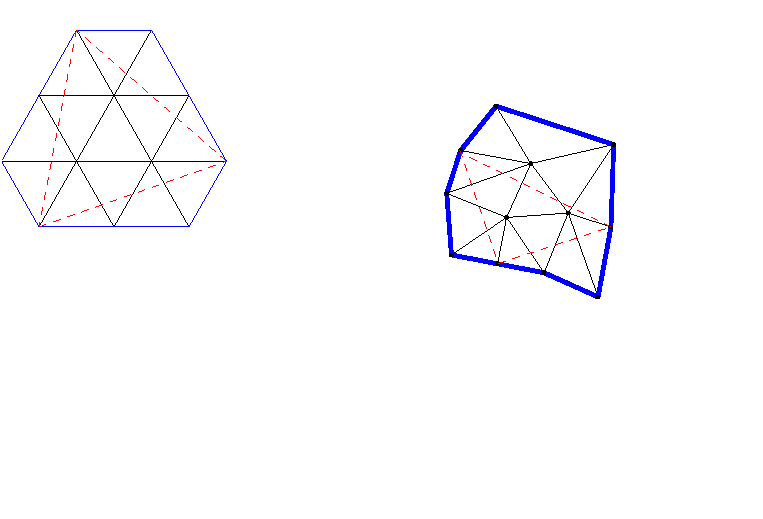
\includegraphics{FigureParam/PL21dualSec1.pdf}}}\par
\end{center}
}

\frame{
  \frametitle{Example of $GC_{2,1}(Cube)$}
\begin{center}
\resizebox{97mm}{!}{\rotatebox{0}{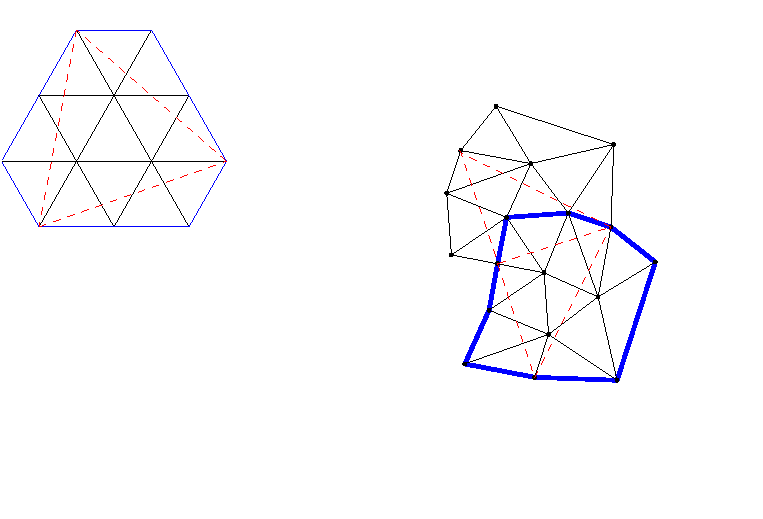
\includegraphics{FigureParam/PL21dualSec2.pdf}}}\par
\end{center}
}

\frame{
  \frametitle{Example of $GC_{2,1}(Cube)$}
\begin{center}
\resizebox{97mm}{!}{\rotatebox{0}{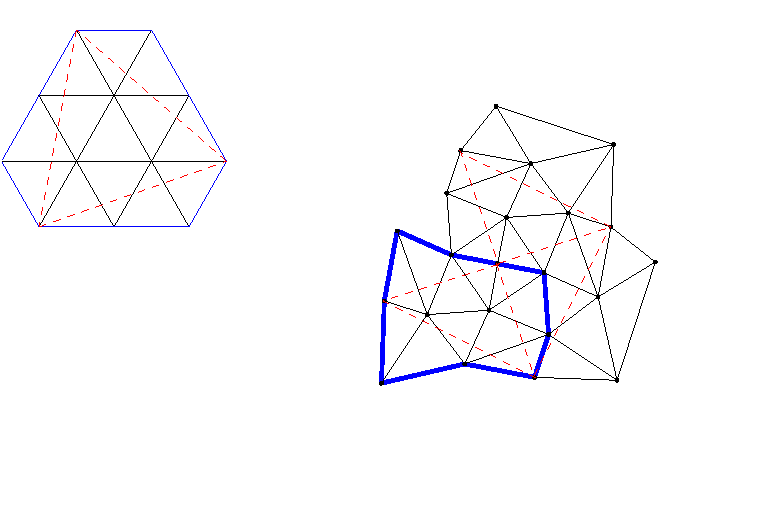
\includegraphics{FigureParam/PL21dualSec3.pdf}}}\par
\end{center}
}

\frame{
  \frametitle{Example of $GC_{2,1}(Cube)$}
\begin{center}
\resizebox{97mm}{!}{\rotatebox{0}{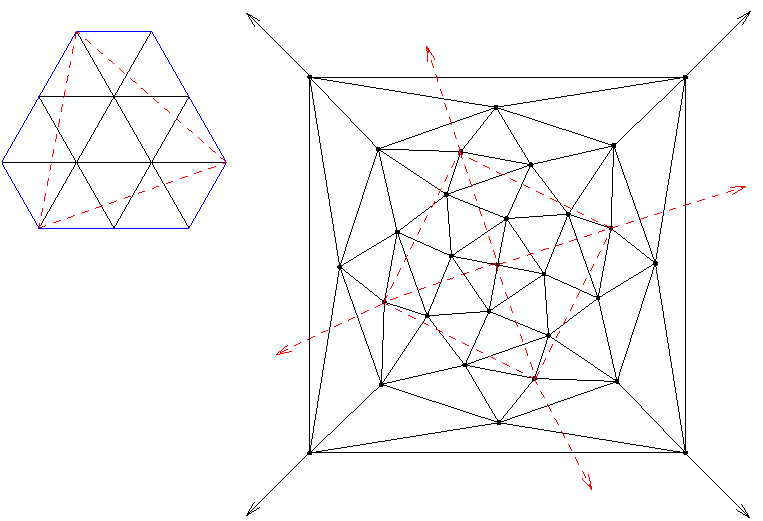
\includegraphics{FigureParam/PL21dualSec4.pdf}}}\par
\end{center}
}

\frame{
  \frametitle{Example of $GC_{2,1}(Cube)$}
\begin{center}
\resizebox{70mm}{!}{\rotatebox{0}{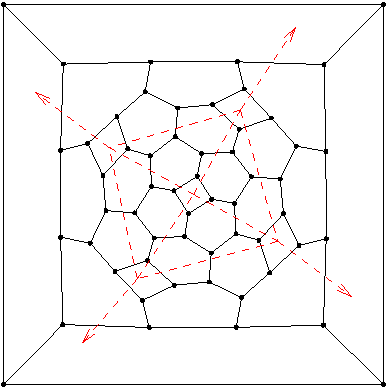
\includegraphics{FigureParam/PL21sec.pdf}}}\par
\end{center}
}





\frame{
  \frametitle{Properties of Goldberg Coxeter construction}

\begin{itemize}
\item It is more convenient to work with the dual.
\item If a fullerene is of symmetry $(I,I_h)$ then it is of the form $GC_{k,l}(Dodecahedron)$ for some $k,l$.\\
      Similarly, if a $(0,6,0)$-, $(4,0,0)$ is of symmetry $(O, O_h)$, $(T, T_d)$ then it is $GC_{k,l}(Cube)$, $GC_{k,l}(Tetrahedron)$.
\begin{itemize}
\item M. Goldberg, {\em A class of multi-symmetric polyhedra}, Tohoku Mathematical Journal {\bf 43} (1937) 104--108.
\end{itemize}
\item It is useful to embed $k,l$ as an Eisenstein integer, i.e. $z=k + l \omega$ with $\omega=e^{i\pi/3}$.
\item $GC_{k,l}(G_0)$ has $(k^2+kl+l^2)|G_0| = |z|^2 |G_0|$ vertices.
\item The parameter symmetry $z\mapsto z \omega^r$ does not change the graph.
\end{itemize}
}


%\frame{
%  \frametitle{The case of $1$ parameter: Goldberg-Coxeter construction}
%
%\begin{itemize}
%\item For a dual fullerene $G$ of symmetry $I$ or $I_h$, there exist two parameters $k$ and $l$ such that $G=GC_{k,l}(Icosahedron)$. Below $GC_{2,1}(Icosahedron)$:
%\end{itemize}
%\begin{center}
%\begin{minipage}[b]{4.3cm}
%\centering
%\resizebox{33mm}{!}{\rotatebox{0}{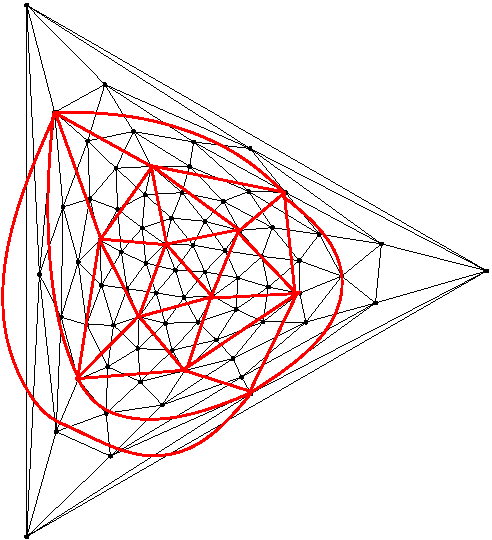
\includegraphics{FigureParam/PLdodec21dualSec.pdf}}}\par
%\end{minipage}
%\end{center}
%\begin{itemize}
%\item The symmetries in the parameters are $(k+l\omega) \mapsto (k+l\omega)\omega^r$
%\end{itemize}
%
%}


\frame{
  \frametitle{One case of $2$ parameters: symmetry $D_5$}

\begin{itemize}
\item The $5$-fold axis has to pass through a vertices of degree $5$. There are $5$ vertices of degree $5$ around it.
\end{itemize}
\begin{center}
\begin{minipage}[b]{7.3cm}
\centering
\resizebox{70mm}{!}{\rotatebox{0}{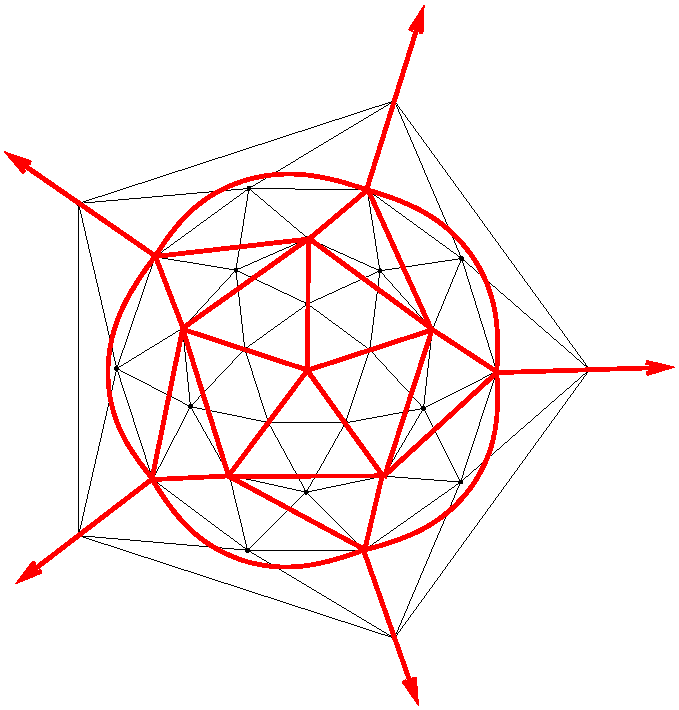
\includegraphics{FigureParam/D5_7bSec.pdf}}}\par
\end{minipage}
\end{center}
}

\frame{
  \frametitle{Parameter symmetries in $D_5$ case}
\begin{center}
\begin{minipage}[b]{9.3cm}
\centering
\resizebox{83mm}{!}{\rotatebox{0}{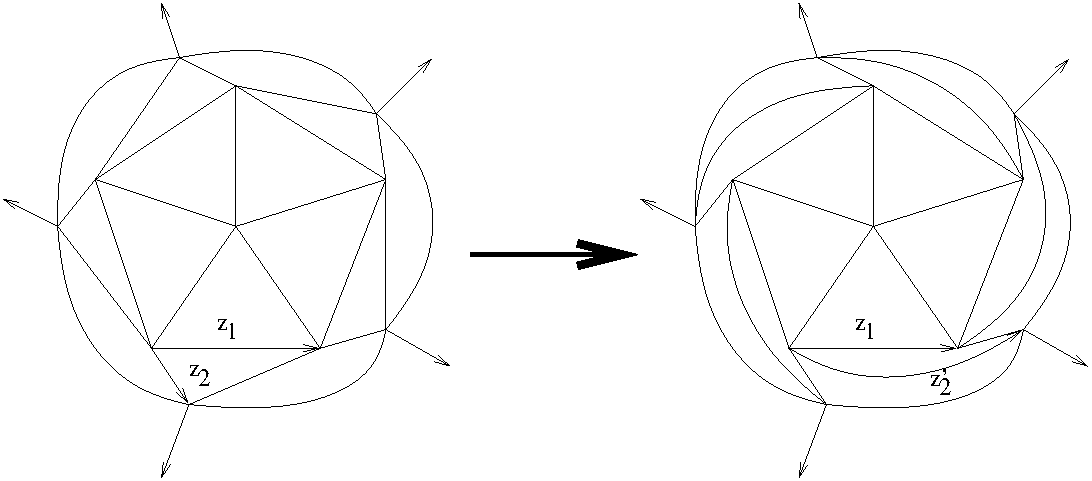
\includegraphics{FigureParam/Transform1.pdf}}}\par
\end{minipage}
\end{center}
\begin{itemize}
\item Operation $1$: $(z_1, z_2)\mapsto (z_1, z_1+z_2)$
\end{itemize}
}

\frame{
  \frametitle{Parameter symmetries in $D_5$ case}
\begin{center}
\begin{minipage}[b]{9.3cm}
\centering
\resizebox{83mm}{!}{\rotatebox{0}{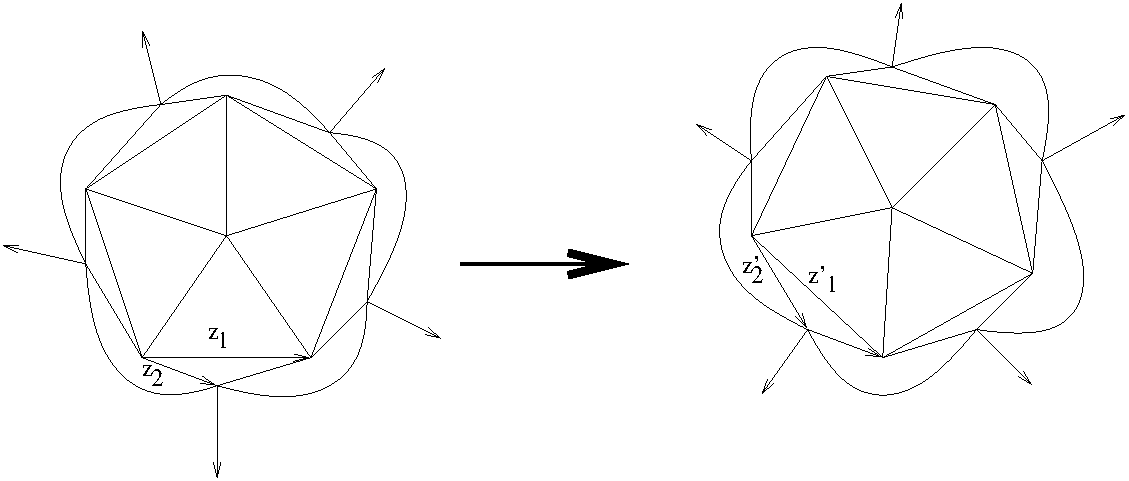
\includegraphics{FigureParam/Transform2.pdf}}}\par
\end{minipage}
\end{center}
\begin{itemize}
\item Operation $2$: $(z_1, z_2)\mapsto (z_1+\omega^2 z_2, z_1 - z_2)$
\item Operation $3$: $(z_1, z_2)\mapsto (z_1,z_2)\omega^r$
\item For a given parameter $(z_1, z_2)$ a graph may not exist.
\item $n_{triangle}(z_1,z_2)=10\{z_1 \overline{z_1} - (z_1\overline{z_2} - \overline{z_1} z_2) (\omega - \overline{\omega})/3\}$.

\end{itemize}


}




\frame{
\begin{center}
{\Huge 
\begin{tabular*}{6cm}{c}
\\[-0.5cm]
\textcolor{blue}{III. }\textcolor{red}{General Thurston}\\
\textcolor{red}{theory}
\end{tabular*}
}
\end{center}
}

\frame{
  \frametitle{Parameterization of $(p_3, p_4, p_5)$-graphs}

\begin{itemize}
\item For a class of $3$-valent plane graph $(p_3, p_4, p_5)$ the number of complex parameters needed to describe it is
\begin{equation*}
m = p_3 + p_4 + p_5 - 2
\end{equation*}
We denote by $z_1, \dots, z_m$ the set of parameters.
\item The number of vertices is expressed as a Hermitian form $q$ in the parameters $(z_1, \dots, z_m)$
\item The signature of $q$ is $(1, m-1)$.
\item Denote by $\HH^{m}$ the cone of $(z_1,\dots, z_m)\in \CC^m$ such that $q(z_1, \dots, z_m)>0$.
\end{itemize}
}

\frame{
  \frametitle{Monodromy group}

\begin{itemize}
\item The set of parameters describing the group is not unique, some operations
generalizing the previous ones occur.
\item The Hermitian form is invariant under those transformations
\item The group defined by them is a monodromy group $M(p_3, p_4, p_5)$:
\begin{itemize}
\item P. Deligne, G.D.  Mostow, 
{\em Monodromy of hypergeometric functions and nonlattice integral monodromy},
Inst. Hautes Études Sci. Publ. Math. {\bf 63} (1986) 5--89.
\item G.D. Mostow, 
{\em Generalized Picard lattices arising from half-integral conditions}, 
Inst. Hautes Études Sci. Publ. Math. {\bf 63} (1986) 91--106.
\end{itemize}
(The groups $M(p_3, p_4, p_5)$ form $18$ of the $94$ discrete such groups)
\item Those monodromy groups are image of the braid group $B_m$ and the invariant form $q$ corresponds to the intersection form on $H^1(S^2 - \{p_1, \dots, p_{m+2}\}, L)$ with $L$ a line bundle.
\item As a consequence $M(p_3, p_4, p_5)$ acts discretely over $\HH^{m}$.
\end{itemize}
}




\frame{
  \frametitle{Representability and covolume}

\begin{itemize}
\item Thurston states that if $z\in \ZZ[\omega]^m$ and $q(z)>0$ then there exists $g\in M(p_4, p_4, p_5)$ such that $g(z_1, \dots, z_m)$ is realizable as a $(p_3, p_4, p_5)$-graph.
\item Thus $\HH^{m}\cap \ZZ[\omega]^{m}$ up to the action of the monodromy group $M(p_3,p_4,p_5)$ is a parameter space for the $(p_3, p_4, p_5)$-graphs.
\item The quotient 
\begin{equation*}
\HH^{m} / (\RR_{>0}\times M(p_3, p_4, p_5))
\end{equation*}
 is of finite covolume.
\item The number of $(p_3, p_4, p_5)$-graphs with $n$ vertices grows like $O(n^{m-1})$.
\begin{itemize}
\item C.H. Sah, {\em A generalized leapfrog for fullerene structures}, Fullerenes Science and Technology {\bf 2-4} (1994) 445--458.
\end{itemize}

\end{itemize}
}

\frame{
  \frametitle{Non-compacity}

\begin{itemize}
\item The quotient $\HH^{m} / (\RR_{>0}\times M(p_3, p_4, p_5))$ is non-compact.
\item But the direction of non-compacity are well understood.
\item They correspond to partition of $(p_3, p_4, p_5)$ faces into two $(p_3^i, p_4^i, p_5^i)$ with $i=1$, $2$ and $3p_3^i+2p_4^i+p_5^i=6$.
\item Geometrically those are nanotubes
\end{itemize}
\begin{center}
\resizebox{50mm}{!}{\rotatebox{0}{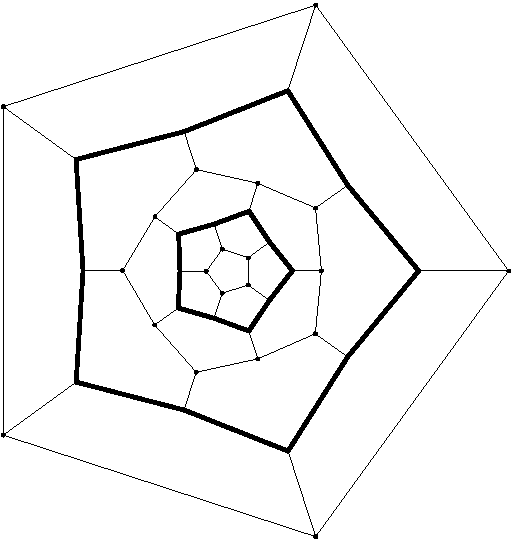
\includegraphics{FigureParam/bD5_2sec.pdf}}}\par
\end{center}
}

\frame{
  \frametitle{Possible generalizations?}
\begin{itemize}
\item We can consider $4$-valent plane graphs. Euler formula for them is 
\begin{equation*}
\sum_{i\geq 3} (4-i) p_i = 8
\end{equation*}
with $p_i$ the number of $i$-gons. A priori those correspond to some Deligne-Mostow orbifolds.
\item What is not clear is how the theory depends on
\begin{itemize}
\item The positive curvature. What can go wrong if $p_7=1$?
\item Parameterization of orientable surfaces. There Euler formula is
\begin{equation*}
\sum_{i\geq 3} (6-i) p_i = 6(2-2g)
\end{equation*}
\end{itemize}
There is no doubt that such parameterization are possible. But what is the geometric structure of the quotient?

\end{itemize}
}


\frame{
\begin{center}
{\Huge 
\begin{tabular*}{8cm}{c}
\\[-0.5cm]
\textcolor{blue}{IV. }\textcolor{red}{Angle description}\\
\end{tabular*}
}
\end{center}
}


\frame{
  \frametitle{Alternative parameterization: by angles}

\begin{itemize}
\item Suppose we have a triangulation of a $2$-dimensional manifold with $t$ triangles. 
\item If we assign the angles of a triangle then the length of the edges is specified up to some multiple. So, we can describe a structure by its angles.
\item The problem is with cycles:
\begin{center}
\begin{minipage}{4.5cm}
\centering
\resizebox{30mm}{!}{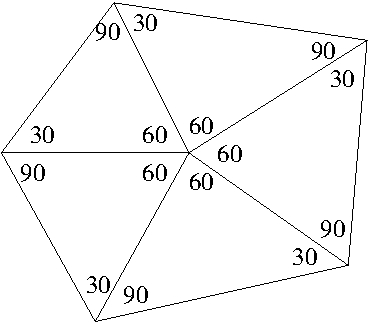
\includegraphics{FigureParam/SomeTriangle.pdf}}\par
\end{minipage}
\end{center}
since going over the cycle we see that only length $0$ is coherent.
\end{itemize}
}

\frame{
  \frametitle{Dihedral angles}
\begin{itemize}
\item For an edge $e$ between two triangles:
\begin{center}
\begin{minipage}{4.5cm}
\centering
\resizebox{30mm}{!}{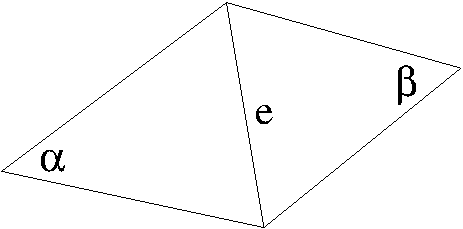
\includegraphics{FigureParam/DihedralAngle.pdf}}\par
\end{minipage}
\end{center}
the dihedral angle is $\pi(e)=\pi - \alpha - \beta$. We can assume $\pi(e)\geq 0$ since otherwise we can switch the edge $e$.
\item For a triangle $t$ of angle $\alpha$, $\beta$, $\gamma$ the hyperbolic volume is:
\begin{equation*}
L(t)=L(\alpha, \beta, \gamma) = L(\alpha) + L(\beta) + L(\gamma)
\end{equation*}
with
\begin{equation*}
L(x) = -\int_0^x \log(2\sin\, t) dt
\end{equation*}
a strictly concave function.
\end{itemize}
}


\frame{
  \frametitle{Rivin's theory}
\begin{itemize}
\item For a triangulation $t_1$, \dots, $t_N$ with a set of
dihedral angles $\Pi=\{\pi(e)\}$ we minimize over the set of all possible angles the sum
\begin{equation*}
\sum_i L(t_i)
\end{equation*}
subject to the constraint that its set of dihedral angles is $\Pi$
\item Necessarily the minimum is unique and is attained by a set of angles all positive.
\item The derivative with respect to angle being $0$ are equivalent to the coherency of the length.
\item So, dihedral angles form a set of parameters. For fullerene this is $18$ parameters.
\item I. Rivin, {\em Euclidean structure on simplicial surfaces and hyperbolic volume}, The Annals of mathematics {\bf 139} (1994) 553--580.
\end{itemize}
}


\frame{
\begin{center}
{\Huge 
\begin{tabular*}{6cm}{c}
\\[-0.5cm]
\textcolor{blue}{V. }\textcolor{red}{Spectrum}\\
\end{tabular*}
}
\end{center}
}


\frame{
  \frametitle{Eigenvalues of graphs}

\begin{itemize}
\item For a $3$-valent plane graph $G$ the adjacency matrix $A$ is a symmetric matrix with
\begin{equation*}
A(i,j)=\left\{\begin{array}{rl}
1 & \mbox{~if~} (i,j) \mbox{~is~an~edge}\\
0 & \mbox{~otherwise}
\end{array}\right.
\end{equation*}
\item $3$ is always an eigenvalue while $-3$ is an eigenvalue if and only if $G$ is bipartite that is has faces of only even size.
\item The infinite plane tiling by hexagon has spectrum $[-3,3]$.
\begin{itemize}
\item P. E. John and H. Sachs,
{\em Spectra of toroidal graphs},
Discrete Mathematics {\bf 309} (2009) 2663.
\end{itemize}
\item This is also the case of infinite nanotubes:
\begin{itemize}
\item L. F. Chibotaru, D. Compernolle and A. Ceulemans, 
{\em Electron transmission through atom-contacted carbon nanotubes},
Physical Review B {\bf 68} (2003) 125412 (31 pp).
\end{itemize}
\end{itemize}
}




\frame{
  \frametitle{General finiteness theorem}

Consider a class of $(p_3, p_4, p_5)$-graphs
\begin{itemize}
\item \textcolor{blue}{Lemma}: If the number $n$ is large enough then a $(p_3, p_4, p_5)$-graph contains
\begin{itemize}
\item a large enough patch of hexagons or
\item a long enough nanotube.
\end{itemize}
\item Two proof methods:
\begin{itemize}
\item One is based on a simple covering argument (by J. Graver).
\item Another on Thuston's parameterizations and the fact that the compactifications of the parameter space are indexed by the partititions of the $5$-gons into two sets of six $5$-gons.
\end{itemize}
\item \textcolor{blue}{Theorem:} For any interval $I=[a,b]\subset [-3, 3]$ with $a<b$ the set of $(p_3,p_4,p_5)$-graphs having no eigenvalue in $I$ is finite.
\begin{itemize}
\item M. Dutour Sikiri\'c and P. Fowler, 
{\em Cubic ramapolyhedra with face size no larger than $6$},
Journal of Mathematical Chemistry {\bf 49} (2011) 843--858.
\end{itemize}

\end{itemize}
}


\frame{
\begin{center}
{\Huge 
\begin{tabular*}{6cm}{c}
\\[-0.5cm]
\textcolor{blue}{VI. }\textcolor{red}{Zigzags}\\
\end{tabular*}
}
\end{center}
}


\frame{
  \frametitle{Definition}
\begin{itemize}
\item In a plane graph a \textcolor{red}{zigzag} is a circuit of edges such that two consecutive share a face and vertex but three do not share a face.
\end{itemize}
\begin{center}
\resizebox{70mm}{!}{\rotatebox{0}{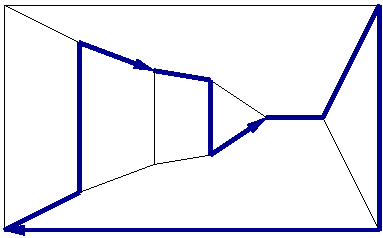
\includegraphics{ZIGZAGpicture/ZigZagSample4naked.pdf}}}\par
\end{center}

}



\frame{
  \frametitle{Zigzag structure of Goldberg Coxeter construction}

\begin{itemize}
\item For a $3$-valent plane graph $G_0$ we define a permutation group $Mov(G_0)$ and two elements $L$ and $R$.
\item The length of zigzags of $GC_{k,l}(G_0)$ is computed from the cycle structure of $L\odot_{k,l} R$:
\begin{itemize}
\item $L \odot_{1,0} R=L$ and $L\odot_{0,1} R=R$.
\item If $gcd(k,l)=1$ then we have 
\begin{equation*}
\left\lbrace\begin{array}{rcrcll}
L\odot_{k,l} R&=&  L   &\odot_{k-ql\mbox{~},\mbox{~}l}&RL^q  &\mbox{if~}k-ql\geq 0\\
L\odot_{k,l} R&=&  R^qL&\odot_{k\mbox{~},\mbox{~} l-qk}&R     &\mbox{if~}l-qk\geq 0
\end{array}\right.
\end{equation*}
The product is defined only up to conjugacy.
\end{itemize}
\item If $gcd(k,l)=m>1$ then we simply multiply the length of zigzags by $m$:
\begin{itemize}
\item M. Dutour and M. Deza, {\em Goldberg-Coxeter construction for $3$- and $4$-valent plane graphs}, Electronic Journal of Combinatorics {\bf 11-1} (2004) R20.
\end{itemize}
\end{itemize}

}


\frame{
  \frametitle{The structure of $(4,0,0)$-graphs}

\begin{center}
\begin{minipage}{5cm}
\centering
\resizebox{5cm}{!}{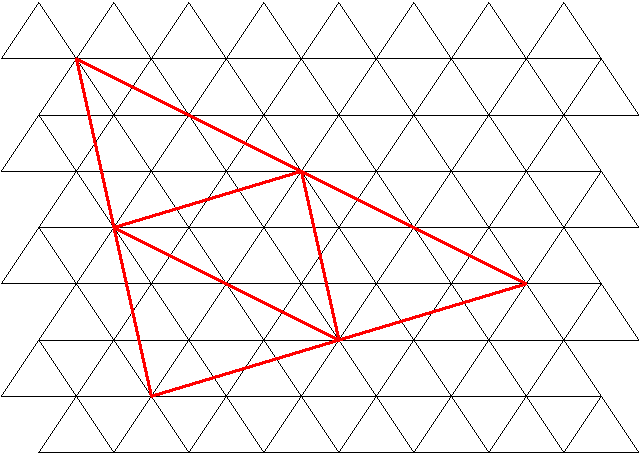
\includegraphics[bb=30 20 260 200, clip]{GOLDBERGpicture/Encoding3n.pdf}}\par
$4$ triangles in $\ZZ[\omega]$
\end{minipage}
\begin{minipage}{5cm}
\centering
\resizebox{5cm}{!}{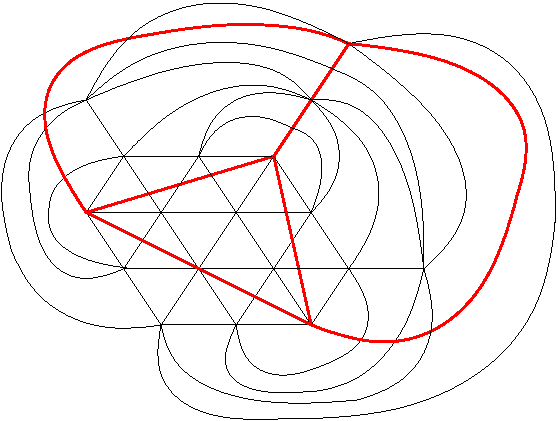
\includegraphics{GOLDBERGpicture/CorrespondingGraph3n.pdf}}\par
The corresponding triangulation
\end{minipage}
\end{center}

\begin{center}
\begin{minipage}{5cm}
\resizebox{3cm}{!}{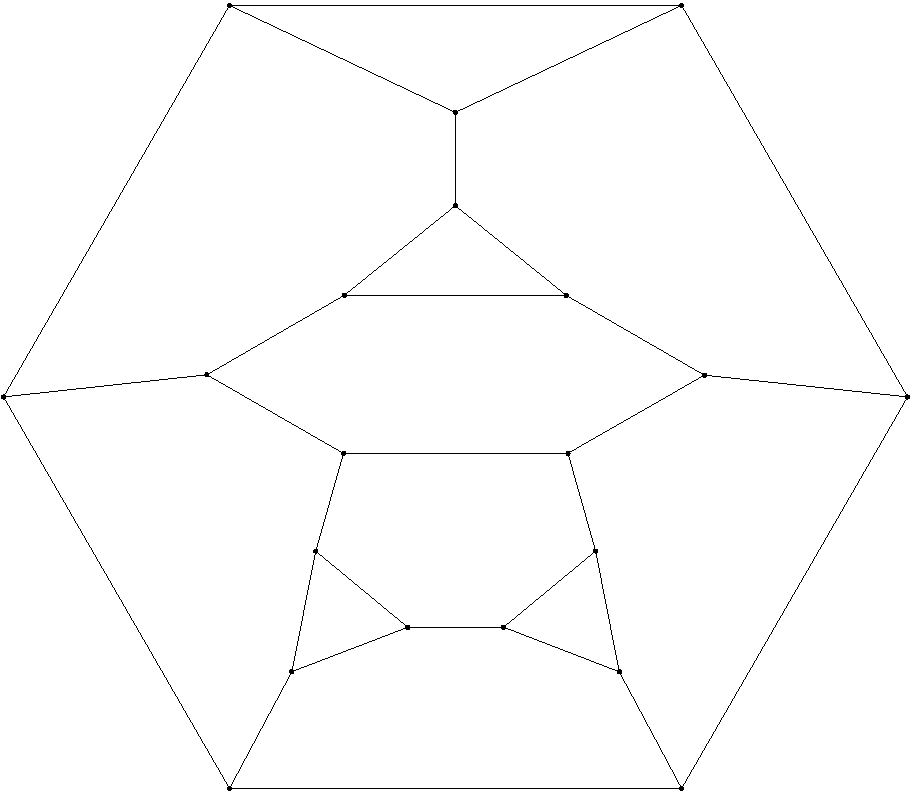
\includegraphics{GOLDBERGpicture/FromTrigSec.pdf}}\par
\end{minipage}
\begin{minipage}{5cm}
\centering
A $(4,0,0)$-graph of symmetry $D_{2d}$
\end{minipage}
\end{center}
}


\frame{
  \frametitle{Zigzags in $(4,0,0)$- and $(0,6,0)$-graphs}

\begin{itemize}
\item All zigzags of $(4,0,0)$-graphs are simple.
\item The vector enumerating length of zigzags of $(4,0,0)$-graphs is
\begin{equation*}
(4s_1)^{m_1}, (4s_2)^{m_2},(4s_3)^{m_3}\mbox{~~~with~~~}s_im_i=\frac{n}{4}.
\end{equation*}
\item \textcolor{red}{Conjecture:} All $(0,6,0)$-graphs with only simple zigzags are:
\begin{itemize}
\item $GC_{k,0}(Cube)$, $GC_{k,k}(Cube)$ and
\item the family of graphs with parameters $(m,i)$ with $n=4m(2m-3i)$ vertices and a vector of zigzags
\begin{equation*}
z=(6m-6i)^{3m-3i}, (6m)^{m-2i}, (12m-18i)^i
\end{equation*}
\end{itemize}
They have symmetry $D_{3d}$ or $O_{h}$ or $D_{6h}$

\end{itemize}
}


\frame{

\vspace{1.5cm}
\begin{center}
{\Huge \textcolor{red}{T}\textcolor{blue}{H}\textcolor{green}{A}\textcolor{blue}{N}\textcolor{red}{K}}\\[1cm]
{\Huge \textcolor{red}{Y}\textcolor{blue}{O}\textcolor{red}{U}}
%\epsfig{file=plit-gal10.eps, height=5.5cm}
\end{center}
}



\end{document}
